\appendix
\chapter{Appendix}

This appendix contains supplementary technical materials for CricketVision, including the complete Git version control commit history log, GitHub repository screenshot, and core backend/frontend source code listings.

\section{Git Version Control Commit History Log}

The source code and project deliverables for CricketVision are managed using Git version control and pushed to the GitHub repository (\texttt{Abhijithmohan10/cricketvision}). Table \ref{tab:appendix_git_log} details the recorded repository commit history leading up to the evaluation phase:

\begin{table}[H]
\centering
\caption{Complete Git Repository Commit Log (\texttt{Abhijithmohan10/cricketvision})}
\label{tab:appendix_git_log}
\begin{tabular}{llll}
\toprule
\textbf{Commit Hash} & \textbf{Date} & \textbf{Author} & \textbf{Commit Message / Deliverable Summary} \\
\midrule
\texttt{c47ef12} & 18/09/2026 & Abhijith Mohan & Add comprehensive official project README.md for CricketVision AI repository \\
\texttt{4d1b4d2} & 18/09/2026 & Abhijith Mohan & Update Scrum Book with Sprint 7 log, US-23 to US-25 deliverables \& story points \\
\texttt{732440f} & 18/09/2026 & Abhijith Mohan & Add Head-to-Head Player Comparison view with dual skill radar overlays \\
\texttt{9faf036} & 09/09/2026 & Abhijith Mohan & Optimize website layout for seamless mobile \& desktop responsiveness \\
\texttt{8e00af0} & 03/09/2026 & Abhijith Mohan & fix: resolve UI bugs (Navbar dropdown, TeamBuilder async load, Chat scroll) \\
\texttt{2898d5a} & 03/09/2026 & Abhijith Mohan & feat: implement strict access controls for Player Portal \& default auth state \\
\texttt{6562e08} & 03/09/2026 & Abhijith Mohan & fix: centralize API URLs and secure JWT secret \\
\texttt{7f37213} & 03/09/2026 & Abhijith Mohan & chore: add environment config and fix Vite base path for GH Pages \\
\texttt{e85cb44} & 24/08/2026 & Abhijith Mohan & feat: add bcrypt auth, JWT tokens, PDF export, mobile responsive CSS \\
\texttt{e6f29fa} & 13/08/2026 & Abhijith Mohan & Fix print preview blank page with React portal \& clean A4 CSS \\
\texttt{bdf8ee8} & 13/08/2026 & Abhijith Mohan & Fix print preview layout to single page A4 \\
\texttt{bc2e426} & 11/08/2026 & Abhijith Mohan & Initial commit \\
\bottomrule
\end{tabular}
\end{table}

Figure \ref{fig:ss_github} shows the actual GitHub repository commit log interface for \texttt{Abhijithmohan10/cricketvision}.

\begin{figure}[H]
\centering
\IfFileExists{screenshots/GitHub_Commits_History.png}{
    \includegraphics[width=0.90\textwidth]{screenshots/GitHub_Commits_History.png}
}{
    \IfFileExists{GitHub_Commits_History.png}{
        \includegraphics[width=0.90\textwidth]{GitHub_Commits_History.png}
    }{
        \fbox{\parbox{0.8\textwidth}{\centering \textbf{[Screenshot: GitHub Repository Commit History]}}}
    }
}
\caption{GitHub Version Control Repository Commit History Screenshot}
\label{fig:ss_github}
\end{figure}

\section{Core Source Code Listings}

\subsection{Backend REST API Server Controllers (\texttt{server.js})}
\begin{lstlisting}[language=Java, caption={Express Server REST Endpoints \& Mongoose Setup}]
const express = require('express');
const mongoose = require('mongoose');
const cors = require('cors');

const app = express();
app.use(cors());
app.use(express.json());

// Connect to Local MongoDB Instance
mongoose.connect('mongodb://127.0.0.1:27017/cricketvision')
  .then(() => console.log('Connected to MongoDB: cricketvision'))
  .catch(err => console.error('MongoDB Connection Error:', err));

// Player REST Endpoints
app.get('/api/players', async (req, res) => {
  try {
    const players = await Player.find({});
    res.json(players);
  } catch (err) {
    res.status(500).json({ error: 'Failed to fetch players' });
  }
});

app.post('/api/players', async (req, res) => {
  try {
    const newPlayer = new Player(req.body);
    await newPlayer.save();
    res.status(201).json(newPlayer);
  } catch (err) {
    res.status(400).json({ error: err.message });
  }
});

app.put('/api/players/:id', async (req, res) => {
  try {
    const updated = await Player.findOneAndUpdate({ id: req.params.id }, req.body, { new: true });
    res.json(updated);
  } catch (err) {
    res.status(400).json({ error: err.message });
  }
});

app.delete('/api/players/:id', async (req, res) => {
  try {
    await Player.deleteOne({ id: req.params.id });
    res.json({ message: 'Player deleted successfully' });
  } catch (err) {
    res.status(500).json({ error: 'Delete failed' });
  }
});
\end{lstlisting}

\subsection{Stochastic Match Simulator Win Probability Logic}
\begin{lstlisting}[language=Java, caption={Win Probability Calculation Formula}]
export function calculateWinProbability(currentOver, targetScore, currentRuns, wicketsLost, pitchFactor, weatherImpact) {
  const oversRemaining = 20 - currentOver;
  const runsNeeded = targetScore - currentRuns;
  const wicketsRemaining = 10 - wicketsLost;

  if (runsNeeded <= 0) return 100;
  if (wicketsRemaining <= 0 || oversRemaining <= 0) return 0;

  const currentRRR = runsNeeded / oversRemaining;
  const currentRR = currentOver > 0 ? currentRuns / currentOver : 6.0;

  const rrrDiff = currentRRR - currentRR;
  
  // Logistic regression exponent formula
  const exponent = -(0.45 * (6.0 - currentRRR) + 0.35 * wicketsRemaining + 0.15 * pitchFactor + 0.05 * weatherImpact);
  const winProb = (1 / (1 + Math.exp(exponent))) * 100;

  return Math.min(Math.max(Math.round(winProb), 1), 99);
}
\end{lstlisting}

\subsection{360° Wagon Wheel Polar Coordinate Transformation}
\begin{lstlisting}[language=Java, caption={Wagon Wheel SVG Coordinate Mapper}]
export function polarToCartesian(centerX, centerY, radius, angleInDegrees) {
  const angleInRadians = (angleInDegrees - 90) * Math.PI / 180.0;
  return {
    x: centerX + (radius * Math.cos(angleInRadians)),
    y: centerY + (radius * Math.sin(angleInRadians))
  };
}
\end{lstlisting}
